\documentclass[11pt,border=5pt]{standalone}
\usepackage{fontspec}
\setmainfont{cmunrm.otf}[BoldFont=cmunbx.otf,ItalicFont=cmunti.otf,BoldItalicFont=cmunbi.otf]
\usepackage{amsmath}
\usepackage{unicode-math}
\setmathfont{NewCMMath-Regular.otf}
\usepackage{tikz}
\usetikzlibrary{arrows.meta,patterns,angles,quotes}
\begin{document}
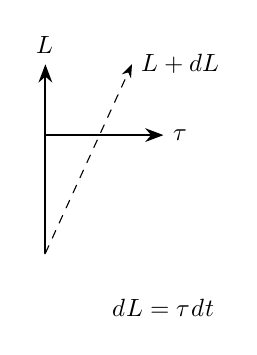
\begin{tikzpicture}[>=Stealth,font=\small,line cap=round,line join=round]
\draw[->,thick] (0,0) -- (0,2.4) node[above] {$L$};
\draw[->,thick] (0,1.5) -- (1.5,1.5) node[right] {$\tau$};
\draw[->,thin,dashed] (0,0) -- (1.1,2.4) node[right] {$L+dL$};
\node at (1.5,-0.7) {$dL=\tau\,dt$};

\end{tikzpicture}
\end{document}
